\documentclass{thomasClass}
\usepackage{amssymb}
\usepackage{multirow}

\title{\textbf{Required Practical 4}
\\An investigation into the effect of temperature on the plasma membrane of plant tissue
}
\author{Thomas Boxall}
\date{February 2021}

\begin{document}

\maketitle

\section{Method}
\begin{enumerate}
    \item Use a cork borer to cut cylinders from the beetroot. Cut these cylinders into lengths of 15mm.
    \item Carefully dry the cut beetroot using a paper towel.
    \item Take 6 test tubes and fill with water $8cm^3$ of distilled water and $2cm^3$ of neutral buffer solution.
    \item Place one test tube in each water bath and leave for five minutes. Check the temperature with a thermometer. \textit{Temperatures should be 10\textdegree C; 20\textdegree C; 30\textdegree C; 45\textdegree C; 60\textdegree C; 85\textdegree C}.
    \item Add a cylinder of beetroot to each tube and leave for 10 minutes.
    \item After 10 minutes, remove the beetroot cylinders from a,, the test tubes, mix the remaining solution. Then with a clean pipette for each tube, take a sample from each of the test tubes and fill 6 cuvettes. Put lids on the cuvettes.
    \item Measure the percentage transmission and absorbance of light at 490, 520 and 550nm (this allows each pigment to be tested) using a colorimeter and record the results in a table.
\end{enumerate}
\section{Results}
\subsection{Class results}
\subsubsection{Data table}
\begin{table}[H]
\centering
\begin{tabularx}{0.8\textwidth}{c|XX|XX|XX}
\multirow{3}{*}{Temperature (C)} & \multicolumn{6}{c}{Wavelength of light (nm)}                                \\
                                 & \multicolumn{2}{c}{490} & \multicolumn{2}{c}{520} & \multicolumn{2}{c}{550} \\
                                 & Abs        & Trans      & Abs        & Trans      & Abs        & Trans      \\
                                 \hline
4                                & 0.18       & 67         & 0.2        & 63         & 0.18       & 66         \\
20                               & 0.28       & 52         & 0.3        & 49         & 0.28       & 52         \\
35                               & 0.28       & 53         & 0.32       & 49         & 0.28       & 53         \\
60                               & 1.07       & 9          & 1.16       & 7          & 0.97       & 11         \\
75                               & 1.33       & 5          & 1.44       & 4          & 1.16       & 7          \\
85                               & 0.93       & 12         & 0.98       & 10         & 0.84       & 14        
\end{tabularx}
\end{table}
\textit{Trans: Transmission of light (\%)}\\
\textit{Abs: Absorbance of light (AU)}

\subsubsection{Graph}
\begin{figure}[H]
    \centering
    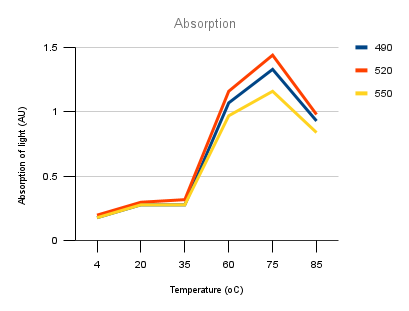
\includegraphics[width=0.7\textwidth]{RPA4-GRAPH1.png}
    \caption{Graph of Absorption}
\end{figure}
\begin{figure}[H]
    \centering
    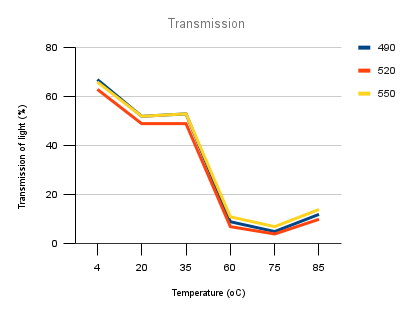
\includegraphics[width=0.7\textwidth]{RPA4-GRAPH2.png}
    \caption{Graph of Transmission}
\end{figure}

\subsection{Exemplar results}
\subsubsection{Data table}
% Please add the following required packages to your document preamble:
% \usepackage{multirow}
\begin{table}[H]
\centering
\begin{tabularx}{0.7\textwidth}{c|cccccccccccc}
\multicolumn{1}{c}{\multirow{2}{*}{Temperature (C)}} & \multicolumn{10}{c}{Transmission (\%)} & \multirow{2}{*}{Mean} \\
\multicolumn{1}{c}{} & \multicolumn{1}{l}{R1} & \multicolumn{1}{l}{R2} & \multicolumn{1}{l}{R3} & \multicolumn{1}{l}{R4} & \multicolumn{1}{l}{R5} & \multicolumn{1}{l}{R6} & \multicolumn{1}{l}{R7} & \multicolumn{1}{l}{R8} & \multicolumn{1}{l}{R9} & \multicolumn{1}{l}{R10} &  \\
35 & 86 & 90 & 90 & 94 & 91 & 83 & 85 & 95 & 96 & 87 & 89.7 \\
40 & 82 & 84 & 85 & 82 & 84 & 84 & 76 & 87 & 82 & 80 & 82.6 \\
55 & 52 & 53 & 53 & 65 & 64 & 53 & 69 & 54 & 42 & 49 & 55.4 \\
65 & 51 & 55 & 54 & 41 & 53 & 33 & 20 & 25 & 36 & 41 & 40.9 \\
75 & 35 & 37 & 38 & 25 & 37 & 41 & 14 & 24 & 16 & 35 & 30.2 \\
80 & 13 & 13 & 14 & 24 & 13 & 17 & 21 & 16 & 17 & 20 & 16.8
\end{tabularx}
\end{table}
\subsubsection{Graph}
\begin{figure}[H]
    \centering
    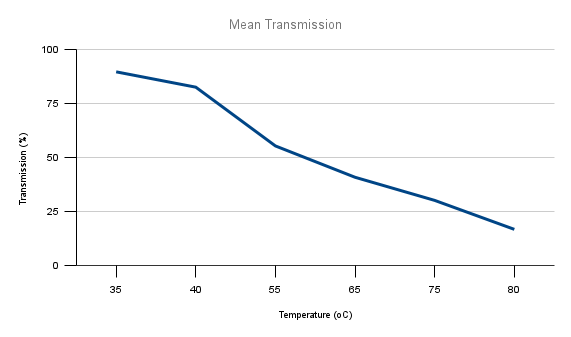
\includegraphics[width=0.7\textwidth]{RPA4-GRAPH3.png}
    \caption{Graph of Transmission}
\end{figure}
\section{Evaluation}
The absorption graph shows that the different wavelengths of light bring out different amounts of pigment at about 60\textdegree C to 75\textdegree C. The graphs show that the more pigment is released at a higher temperature (75\textdegree C) because there is most absorption of with and the least transmission of light. This shows that a temperature of 75\textdegree C is the most effective temperature for breaking a plasma membrane. This is because the temperature causes the proteins in the membrane to break down, creating for holes for the betalin to move through at an accelerated speed because they have a higher kinetic energy as a result of the increased temperature.
\end{document}
